\section{Background}
\label{sec:background}

%This section provides some background information on how
%SSU-ALIGN aligns SSU sequences and how it identifies and removes
%columns from (masks) those alignments that are most likely to contain
%errors in preparation for phylogenetic analysis.  

\subsection{Profile versus nearest neighbor alignment strategies}

There are several existing software packages dedicated to
SSU alignment, including, but not limited to, NAST
\cite{DeSantis06} (used by the GREENGENES database
\cite{DeSantis06a}), PYNAST \cite{Caporaso10},
SINA (used by the SILVA database
\cite{Pruesse07}), and MOTHUR \cite{Schloss09}.
Most of these methods use a \emph{nearest-neighbor}
(NN) based alignment strategy: given a new target sequence to align,
each sequence in a reference alignment is evaluated to find one or
more nearest-neighbor template sequences that are most similar to the
target. An alignment of the target sequence to its template(s) is then
computed, and this alignment is used to place the target within the
context of the full reference alignment (figure~\ref{fig:nnprof}).

In contrast, SSU-ALIGN uses a profile-based alignment
strategy: each target sequence is aligned independently to a
statistical model called a profile
(figure~\ref{fig:nnprof}). The profiles SSU-ALIGN uses for
alignment are called covariance models (CMs)
%, which model both the
%conserved sequence and secondary structure of SSU
\footnote{SSU-ALIGN actually uses two types of profiles,
  CMs and profile HMMs, which model only conserved primary
  sequence. Profile HMMs are used to determine which domain each
  sequence belongs to, and then the corresponding domain-specific CM
  is used to align the sequence, as depicted in
  figure~\ref{fig:strategy}.}.
A comprehensive explanation of CMs is outside the scope of this
guide. Instead, a brief discussion of some of their relevant features
for using SSU-ALIGN and understanding its output is included
below. For more information on CMs see
\cite{Eddy94,Durbin98,Eddy02b,NawrockiEddy07,Nawrocki09,Nawrocki09b,KolbeEddy09}.

\begin{figure}[hb]
  \begin{center}
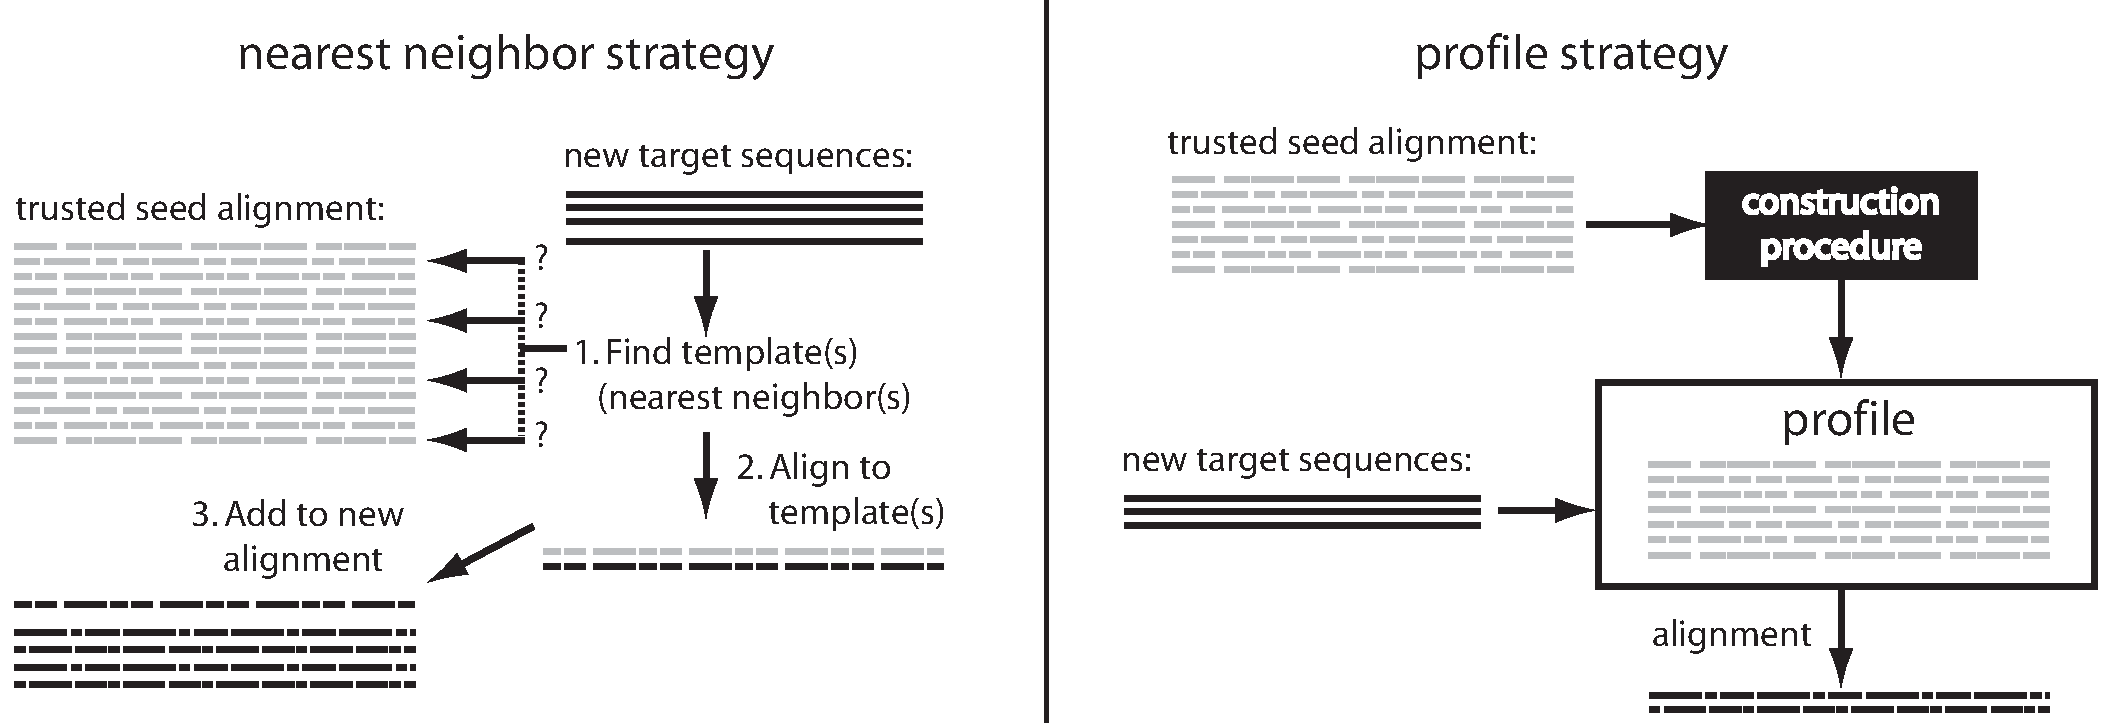
\includegraphics[width=6in]{Figures/nnprof}
  \end{center}
  \caption{Schematic of nearest-neighbor and
        profile based alignment strategies.}
  \label{fig:nnprof}
\end{figure}

\subsubsection{Covariance models: profiles of RNA sequence and secondary structure}

A CM is a consensus model of the conserved sequence and secondary
structure of an RNA family that is built from a multiple sequence
alignment. This alignment is called the \emph{seed}
alignment of the model. The seed alignment should
include a representative set of sequences from the family being
modeled and must include consensus structure annotation indicating
which positions in the alignment are basepaired to each other.  Given
a new target sequence, its best-scoring alignment to the CM can be
computed using a dynamic programming algorithm. Both primary
sequence conservation and secondary structure conservation between the target
and the model contribute to the alignment score.
%  that takes into account both the sequence and structure conservation in the
Figure~\ref{fig:toyex} depicts the building of a CM for a small,
made-up RNA family and the alignment of sequences using that CM.

%The default archaeal, bacterial, and eukaryotic CMs used by
%SSU-ALIGN have 1508, 1582, and 1881 consensus positions,
%respectively. Any column for which fewer than 80\% of the sequences in
%the seed alignment had gaps was defined as a consensus position when
%the default models were constructed\footnote{The 80\% value differs
% from the 50\% default used by the \prog{cmbuild} program of
%  INFERNAL and the RFAM database when building CMs.}.
%The derivation of the three seed alignments and the specific method
%used to build the models is discussed in detail in
%section~\ref{sec:models} of this guide.

%Profiles like CMs use position-specific scores learned from the seed
%alignment for aligning each possible nucleotide in a target sequence
%to each consensus position. Basepaired positions 
%%For example, a consensus position that is
%%100\% \prog{G} in the seed alignment will assign \prog{G} a high
%%score and other nucleotides a low score, while a consensus position
%%that is 25\% \prog{A}, \prog{C}, \prog{G} and \prog{U} will assign all
%%four nucleotides marginal scores. 
%A CM also contains position-specific scores for inserting nucleotides,
%i.e. placing them in between two adjacent consensus positions, and deleting nucleotides,
%i.e. aligning a consensus position to a gap in the sequence. 
%%Whenever
%%a sequence requires an insert after a consensus column, gaps must be
%%added to accomodate that insert in the other sequences in the
%%alignment.

\begin{figure}
\begin{center}
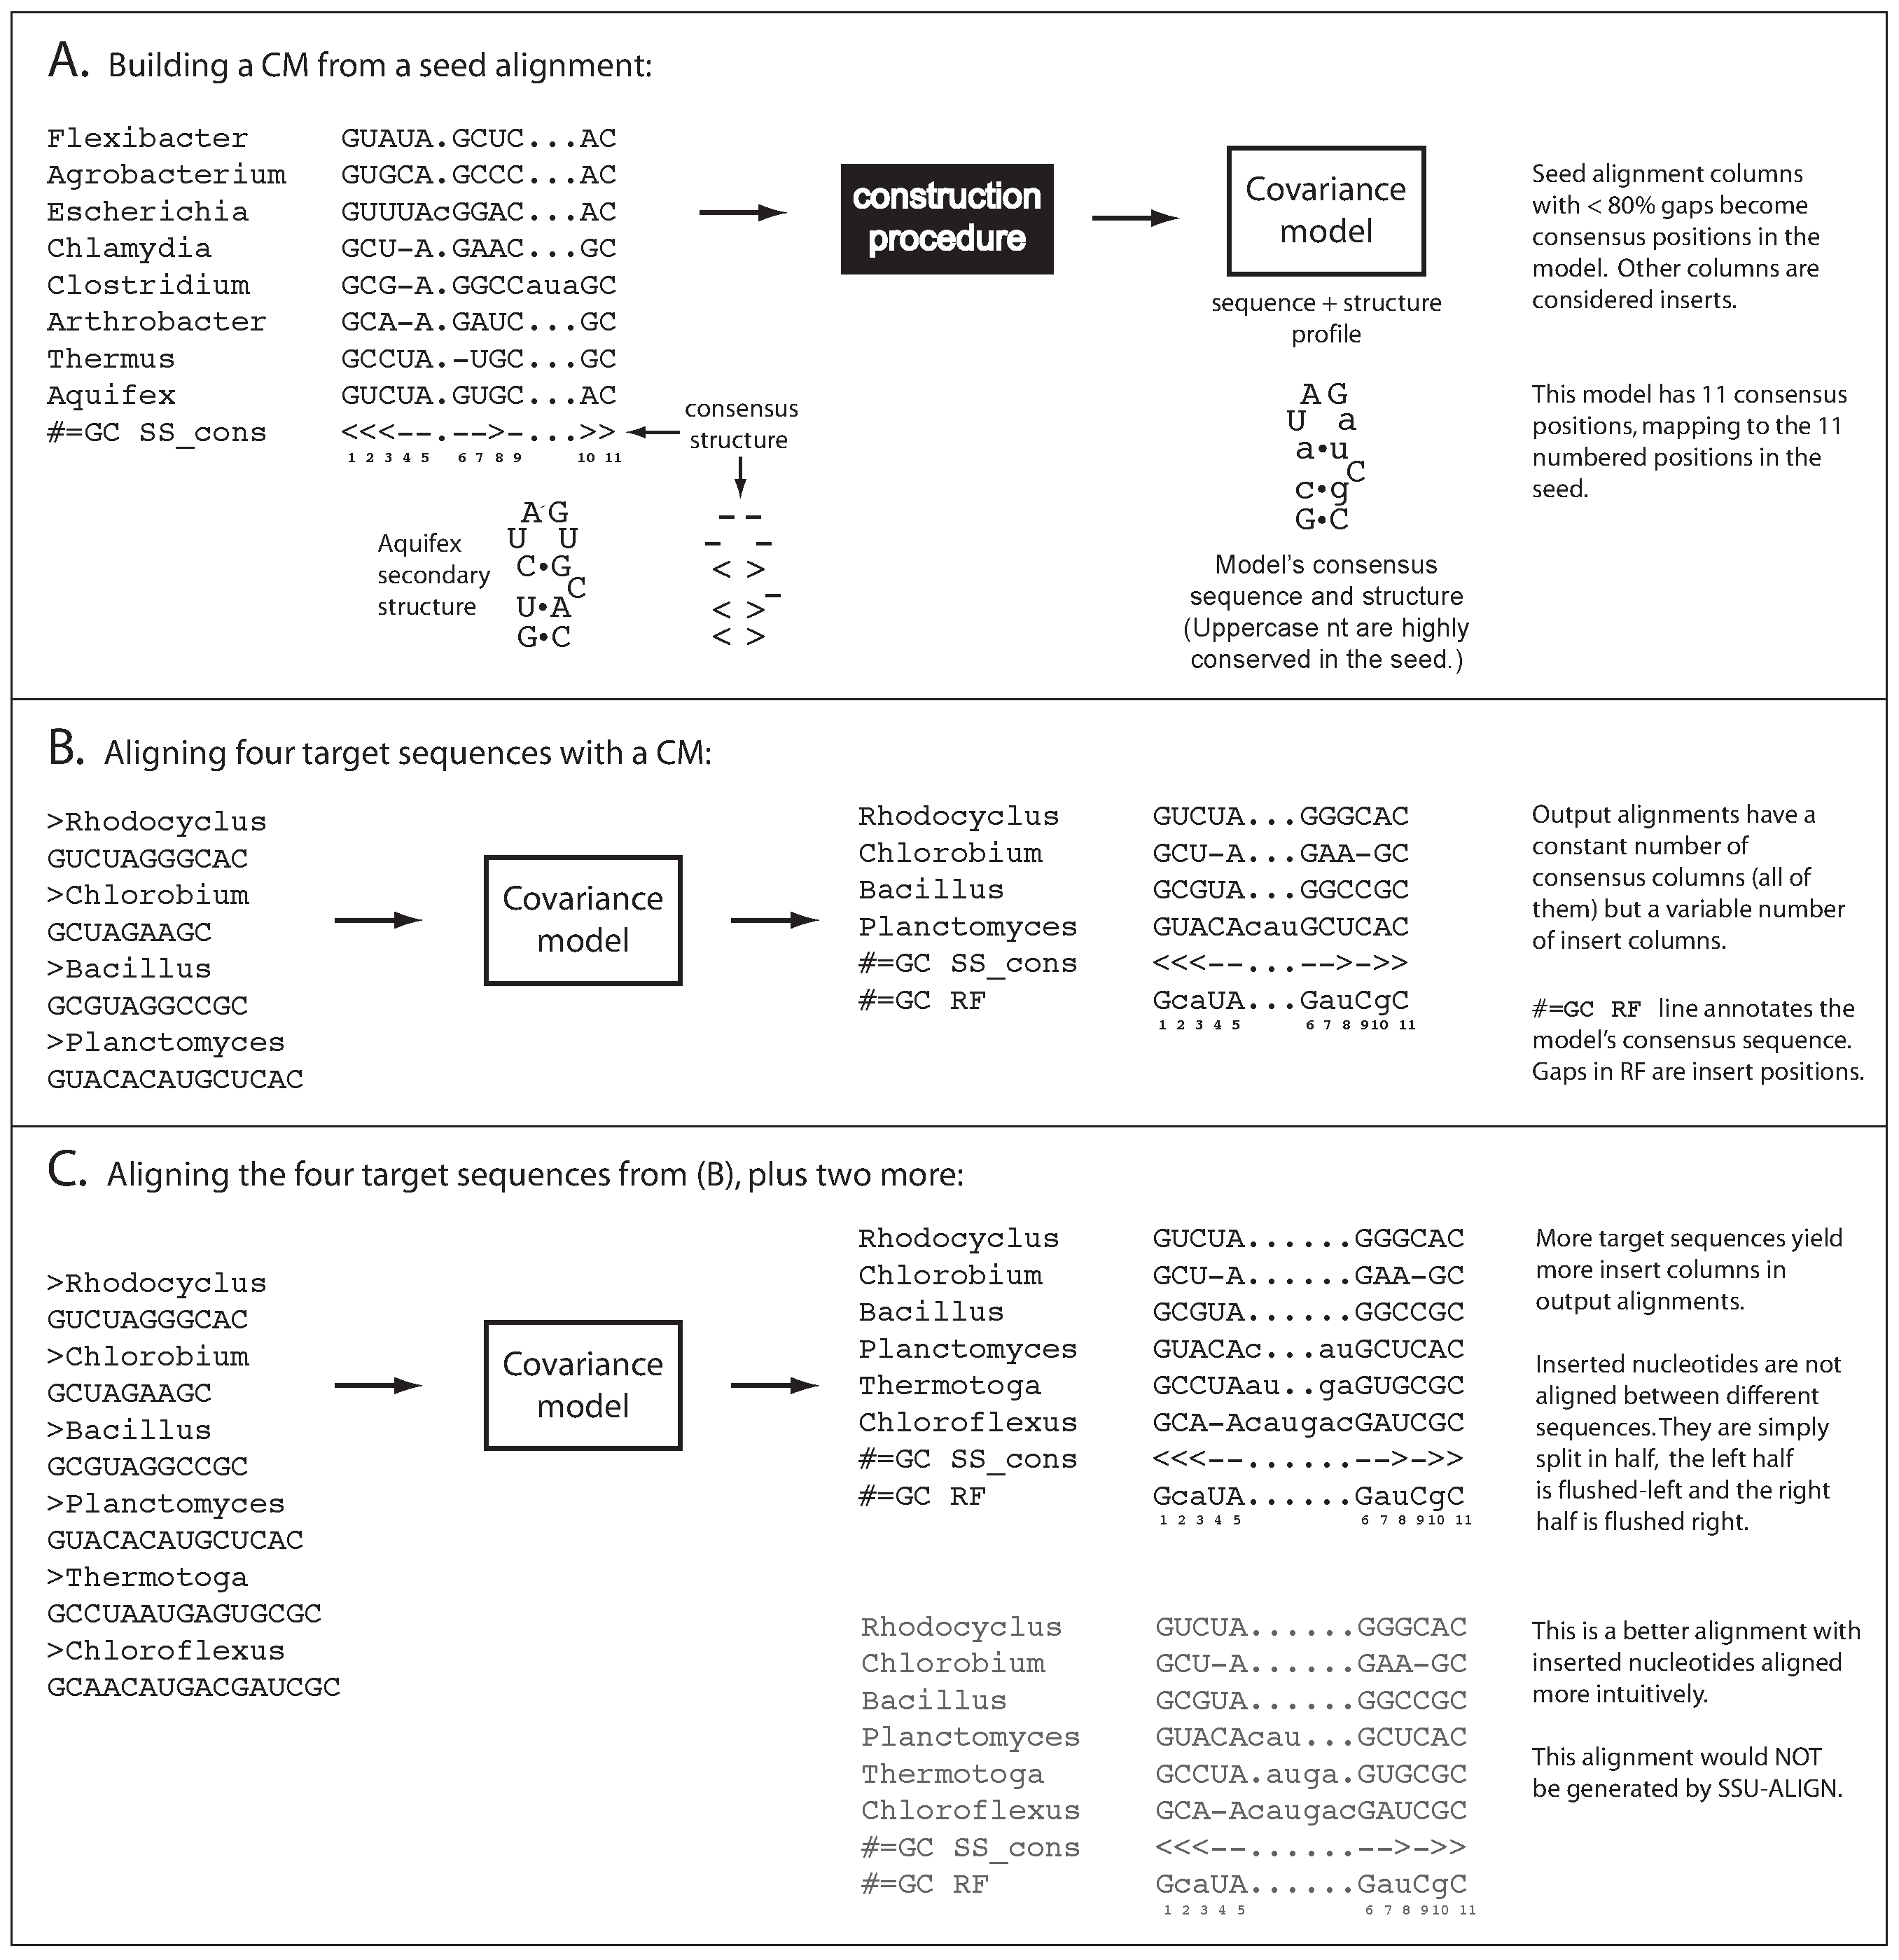
\includegraphics[width=6.1in]{Figures/sa-toy-example}
\end{center}
\caption{\textbf{Building and aligning sequences to an example CM.}
  (A) The made-up seed alignment of 8 homologs of a small stem-loop RNA
family is sent through the black-box construction procedure to create
a CM that models the family. The \prog{\#=GC SS\_cons} line annotates
the consensus structure as shown. Columns that are \prog{.} characters
in this line that have more than 80\% gaps and so are defined as insert
columns. All other columns become consensus positions of the
model. (B) Four unaligned target sequences
are aligned to the CM to generate a new structure annotated
alignment that includes all 11 consensus columns and 3 insert
columns. (C) Six unaligned target sequences, including the same 4 from
(B), are aligned to the CM to generate a new alignment that includes
all 11 consensus columns and 5 insert columns. Nucleotides in insert
columns are not aligned between different sequences, but are simply
split and flushed left and right. The bottom alignment has the
inserted nucleotides aligned more reasonably, but would not be created
by SSU-ALIGN}.
\label{fig:toyex}
\end{figure}

\subsubsection{Profiles use position-specific scores}

The scores used when aligning sequences to a CM are position-specific
and are derived from the observed nucleotide distributions in the seed
alignment. As a simple example, consider the small structural RNA
family in figure~\ref{fig:toyex}. This RNA forms the simple stem-loop
structure shown in part A of the figure. The seed alignment is in
Stockholm format. The \prog{\#=GC SS\_cons} line maps the secondary
structure onto the alignment. Basepairs in this line are indicated by
matching \prog{<} with \prog{>}, just like matching parentheses in a mathematical
formula. When a CM is built from this seed alignment, each of the
columns that include fewer than 80\% gaps will become consensus
positions of the model. There are 11 such positions in the seed
alignment, which are numbered. Other columns are considered insert columns;
these are marked with a \prog{.} in the \prog{\#=GC SS\_cons} line, and
\prog{.} or lowercase nucleotides in the sequences. Basepaired
positions in the structure will become consensus basepairs, and other
positions will be single-stranded consensus positions. 

Each single-stranded consensus position of the model will include
scores for aligning to each of the four possible nucleotides:
\prog{A}, \prog{C}, \prog{G}, and \prog{U}, based on their frequency
in the corresponding position of the alignment. For example, column 5
includes an \prog{A} in all 8 sequences in the seed alignment and so
would assign high scores to \prog{A} and low scores to the \prog{C},
\prog{G}, and \prog{U}. In contrast, column 7, which includes 2 cases of each
of the 4 nucleotides would assign equal, marginal scores to all
4.  

Importantly, basepaired positions will assign
scores to two nucleotides at once and so will include scores for each
of the 16 possible pairs of nucleotides. For example, the pair between
positions 1 and 11 is 100\% \prog{GC} in the seed alignment and so
\prog{GC} pairs in the target would receive high scores, while the
other 15 possible pairs would receive low scores. In contrast, the
pair between positions 3 and 8 includes two of each of the four
possible Watson-Crick basepairs: \prog{AU}, \prog{UA}, \prog{CG}, and
\prog{GC}, and so these four basepairs would receive high scores,
while the other 12 possible pairs would receive lower
scores. 

Additionally, position-specific scores for inserting nucleotides are
derived from the alignment. The only insertions in the seed alignment
occur after positions 5 and 9, and so the score for inserts after
those positions would be higher than for the other
positions. Similarly, the only deletions, i.e. gaps in consensus
positions, occur at positions 4 and 6, with one occuring in 6, and
three in 4. Consequently, the deletion score for position 6 would be
the highest, 4 would be second highest, and all other
positions would receive lower scores. 
(I should point out that this discussion of CM parameterization is
oversimplified for brevity. For formulas and more details, see
\cite{Eddy94,Durbin98,Nawrocki09}.)

In contrast, nearest-neighbor based methods often do not use
position-specific scores. For example, if a single template sequence
is used,  aligning an \prog{A} in the target to any \prog{A} in the
template sequence will receive an identical score. This is because, given
one template sequence, there is no way for the method to distinguish
the relative level of conservation at different positions.
This type of pairwise alignment with position-independent scores is
accurate when the template is nearly identical to the target, but
becomes more difficult as that identity decreases. As a result, most
nearest-neighbor based methods use very large reference alignments
(thousands of sequences) to increase the probability that a nearly
identical template exists for any potential target. Ensuring the
accuracy of such large reference alignments is critical 
but time-consuming and requires expert curators. 
Seed alignments for profile-based methods on the other
traditionally include less than one hundred sequences
\cite{Finn10,Gardner09}.
%In fact, the
%PFAM and RFAM databases collectively include over 12,000
%separate seed alignments, the vast majority of which contain fewer
%than 100 sequences. 

\subsection{Two types of alignment columns: consensus and inserts}
\label{sec:background-columns}

Alignments created by SSU-ALIGN will contain two types of
columns: consensus columns, that correspond to a consensus position of
the model, and insert columns, which include nucleotides inserted
between consensus positions of the model. These columns can be
distinguished based on the \prog{\#=GC RF} line in the alignment
files. Continuing with the small RNA example, figure~\ref{fig:toyex}
shows an alignment of 4 target sequences (part B) and 6 target
sequences (part C) to the CM. Notice that for both alignments, the
\prog{\#=GC RF} line contains 11 nucleotides, one for each of the
consensus columns in the model. These are the highest scoring
nucleotides at each position. Uppercase letters in this line were
highly conserved in the seed alignment, lowercase letters were less
well conserved. Positions that are gaps in the \prog{\#=GC RF} line
contain inserted nucleotides that don't align to any of the consensus
positions. 
SSU-ALIGN alignments created with the same CM will
always include the same number of consensus columns, but the number of
insert columns will vary depending on the input sequences.

There are two important caveats regarding how CMs and SSU-ALIGN
treat inserts:

\begin{enumerate}
\item 
Nucleotides in insert columns are simply inserted, not aligned.

You might have noticed that in part (C) of figure~\ref{fig:toyex}, the
nucleotides in the insert columns after consensus position 5 obviously
misaligned with respect to each other. This is because SSU-ALIGN
does not align inserted nucleotides between different
sequences. Instead, inserted nucleotides are simply split in half, the
left half is placed flush-left next to nearest consensus column on the
left (\prog{au} in \prog{Thermatoga}), and the right half is placed
flush-right next to the nearest consensus column to the right
(\prog{ga} in \prog{Thermatoga}). 

This is an important limitation of
profile-based alignment (at least as implemented in INFERNAL and
SSU-ALIGN). In contrast, a nearest-neighbor based method might
be able to correctly align nucleotides that would be inserts for a
profile. However, inserted positions should be rare. Remember that
consensus positions were defined as any position that had a nucleotide
in at least 20\% of the seed sequences, so if the seed was
representative the most common inserts should only appear in about
20\% of sequences. And if the alignment will eventually be used for
phylogenetic inference, inserted columns in SSU-ALIGN alignments
should be removed first anyway, and so are unimportant. 
It could be argued that the corresponding columns in NN-based
alignments could be kept for phylogenetic inference, but inserts tend
to occur at highly variable regions that are inherently difficult to
correctly align, and so including them might confound phylogenetic
inference that rely on correct alignments. This is
discussed further below in the section on masking alignments.

\item 
Deeper alignments tend to have more insert columns. 

Because the likelihood of a large insertion in at least one sequence
increases as more sequences are added, alignments of large numbers of
sequences (deep alignments) tend to have a lot of insert columns. In
fact, the number of insert columns can be much greater than the number
of consensus columns. Table~\ref{tbl:ttimes} in
section~\ref{sec:stats} provides examples of the dominance of insert
columns in very deep alignments containing more than 100,000

This contrasts markedly with the popular nearest-neighbor based
aligners NAST and SINA, which generate alignments of a
fixed with (7,682 columns for NAST and 50,000 for
SINA). However, to guarantee a fixed width, NAST must
deliberately introduce errors in the alignment in some cases
\cite{DeSantis06}. One reason for doing this is consistency across
datasets: column $x$ from dataset A is directly comparable to column
$x$ from datasets B and C. Importantly, SSU-ALIGN alignments
have a fixed number of \emph{consensus} columns, which facilitates this
type of cross-dataset comparison for consensus positions.
\end{enumerate} 

\subsection{Alignment posterior probabilities are confidence estimates}
\label{sec:background-pp}

When a sequence is aligned to a CM, the posterior probability that each
nucleotide aligns to each position of the model is calculated.  The
posterior probability values for the output alignment are annotated in
the alignment file. These probabilities are \emph{confidence
  estimates} that each nucleotide is correctly aligned, given the
parameters of the CM. The estimates are useful for identifying and
removing columns of the alignment that are most likely to contain
errors. This procedure is called alignment \emph{masking}. Masking is
especially important prior to using the alignment as input to a
phylogenetic inference program because those programs typically assume
that all nucleotides in a given alignment column are homologous and so
are confounded by alignment errors. \prog{ssu-align} output alignments
include posterior probabilities that can be used to automatically
construct and apply masks using the \prog{ssu-mask} program. The
tutorial (section~\ref{sec:tutorial-masking},
page~\pageref{sec:tutorial-masking}) includes an example of alignment
masking.

\subsubsection{Inserted columns should always be excluded during masking}

Importantly, any CM alignment mask should automatically exclude every
insert column of the alignment. This is because, as discussed earlier,
CMs do not actually align inserted nucleotides between different
sequences, but rather simply insert them between the appropriate
consensus columns in the alignment (figure~\ref{fig:toyex}, parts B
and C). This means that sequence nucleotides appearing in the same
insert alignment columns are not aligned with respect to each other
and consequently should be removed prior to phylogenetic analysis
which assumes aligned nucleotides are homologous.  \prog{ssu-mask}
always automatically removes all insert columns from alignments.

\subsubsection{Consensus columns with low alignment confidence should
  also be removed during masking}

It is necessary but not sufficient to remove insert columns
during masking. Additionally, some consensus columns may include
a significant number of nucleotides aligned with low confidence
estimates and these should be removed as well. 

Low alignment confidence tends to occur at positions with low sequence
conservation where insertions and deletions are common, 
corresponding to regions of the molecule that exhibit high length
heterogeneity across different species. 
In such cases, the correct alignment is often ambiguous.
Take for example the CM alignment
of the {\tt GUAU} subsequence of the \emph{Desulfovibrio
desulfuricans} SSU target sequence to a loop region depicted in
figure~\ref{fig:ambiguity}. The reference sequence (this is the
majority-rule consensus sequence from the seed alignment) for the
loop ({\tt AUUCAAC}) differs from {\tt GUAU} in both sequence and
length. Consequently, the CM alignment for this loop is not well
defined, and two alternative alignments are given posterior
probabilities of $0.4$ or higher.  In contrast, the surrounding helix
region, for which higher sequence similarity exists between the
reference and target sequence, is aligned confidently with high
posterior probabilities.

%Additional examples of the correlation between length heterogeneity
%and low alignment confidence are shown in figures~\ref{fig:mask-arc},
%\ref{fig:mask-bac} and \ref{fig:mask-euk}. These masks were derived as
%described in section~\ref{sec:masks}.

\begin{figure}
\footnotesize
\begin{center}
%ORIGINAL DATA is from Macbook: 
%/Users/nawrockie/school/notebook/9_0309_ths/latex/ssu/ambiguity_example
\begin{tabular}{ll}
\tt{00904::Desulfovibrio\_desulfuricans-1} &                         \tt{GAUGUCGGGGA--GUAU---UCUUCGGUGUC} \\
\tt{\#=GR 00904::Desulfovibrio\_desulfuricans-1 PP}  &               \tt{***********--6666---9**********} \\
& \\
\tt{00904::Desulfovibrio\_desulfuricans-2}          &                \tt{GAUGUCGGGGA---GUAU--UCUUCGGUGUC} \\
\tt{\#=GR 00904::Desulfovibrio\_desulfuricans-2 PP} &                \tt{***********---4444--9**********} \\
& \\
\tt{\#=GC SS\_cons}                        &                         \tt{<<<<<<<<<<<<.......>>>>>>>>>>>>} \\
\tt{\#=GC RF}                              &                         \tt{GGUGUuGGgggcAuUcaACgcccUCaGUGCC} \\
\end{tabular}

\vspace{0.2in}
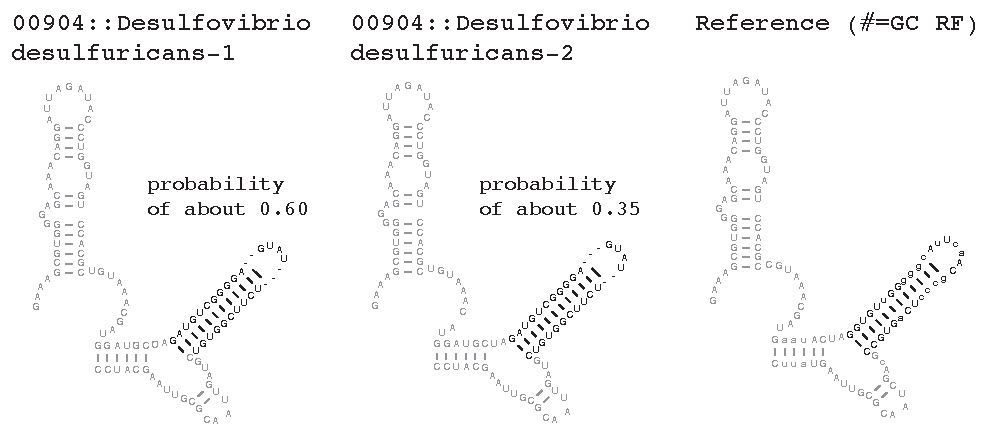
\includegraphics[width=5.7in]{Figures/ambiguity}
\caption[Example of alignment ambiguity in a hairpin loop.]{
  \textbf{Example of alignment ambiguity in a hairpin loop.}  Top: An
  alignment fragment of two different alignments of the
  \emph{Desulfovibrio desulfuricans} (sequence accession
  \texttt{M34113}) sequence from the SSU-ALIGN bacterial seed
  alignment for the region between consensus columns $861$ and $881$.
  Each alignment is annotated with its posterior probability in the
  \texttt{\#=GR PP} rows.  Characters in PP rows have 12 possible
  values: "0-9", "*", or ".". If ".", the position corresponds to a
  gap in the sequence. A value of "0" indicates a posterior
  probability of between 0.0 and 0.05, "1" indicates between 0.05 and
  0.15, "2" indicates between 0.15 and 0.25 and so on up to "9" which
  indicates between 0.85 and 0.95. A value of "*" indicates a
  posterior probability of between 0.95 and 1.0. Higher posterior
  probabilities correspond to greater confidence that the aligned
  nucleotide belongs where it appears in the alignment.  For example,
  the second \texttt{A} in the first aligned sequence has a PP value
  of '6' indicating a posterior probability of between 0.55 and 0.65
  of being aligned in its current position. The
  probability this \texttt{A} aligns in the next position over, as it
  does in the second alignment, is between 0.35 and 0.45 as indicated
  by the 4 in that position.  The \texttt{\#=GC
  SS\_cons} and \texttt{\#=GC RF} rows correspond to the consensus
  secondary structure and sequence respectively.  
%The alignments were
%  created using \texttt{cmalign} to align this sequence to the
%  bacterial CM with the \texttt{--sample} option.  
  Bottom: The
  secondary structures corresponding to the two possible alignments of
  the \emph{D. desulfuricans} and the reference alignment.  Nucleotides
  in the actual alignment are black. Nucleotides surrounding the
  alignment fragment are gray.}
\label{fig:ambiguity}
\end{center}
\end{figure}

\subsubsection{Automated probabilistic masking with \prog{ssu-mask}}

The default masking strategy used by \prog{ssu-mask} is to remove all
insert columns and any consensus column \emph{x} for which fewer than 95\% of
the sequences that are nongaps in \emph{x} have a posterior
probability of less than 0.95 (i.e. any value in the \prog{PP}
annotation that is not \prog{*}). Columns that are 100\% gaps are also
removed. These thresholds were chosen based on good performance using
a simple SSU alignment benchmark. See chapter 9 of \cite{Nawrocki09} for
benchmark details. The thresholds can be changed with the \prog{--pf} and
\prog{--pt} options to \prog{ssu-mask}. Additionally, columns that include
greater than a given fraction of gaps can also be removed using the
\prog{--gapthresh} option. See the \prog{ssu-mask} manual page at the
end of this guide for more details.

Alternatively, it can be useful to apply a preset mask that is not
alignment-specific so that alignments of different datasets can be
directly compared. SSU-ALIGN includes a default preset mask for
each of the default archaeal, bacterial, and eukaryotic
alignments. The determination of these is discussed in
section~\ref{sec:masks}. They can be applied within the
\prog{ssu-mask} program using the \prog{-d} option.

\subsection{Other useful references}

For more information on CM parameterization and alignment, see the
INFERNAL user's guide \cite{infernalguide}.  My
Ph.D. thesis (\htmladdnormallink{http://selab.janelia.org/publications.html}{http://selab.janelia.org/publications.html})
includes more background on SSU databases, alignment methods, CM
acceleration heuristics used by SSU-ALIGN, and the masking
benchmark mentioned earlier. Other useful references on CMs include
\cite{Eddy94,Eddy02b,NawrockiEddy07,Nawrocki09,KolbeEddy09}. Finally,
publications related to the RFAM database
(\htmladdnormallink{http://rfam.sanger.ac.uk/}{http://rfam.sanger.ac.uk/}),
which uses INFERNAL to search for and align structural RNAs
using more than 1000 different CMs, may be of interest
\cite{Griffiths-Jones03,Griffiths-Jones05,Gardner09}.


